\documentclass[a4paper,12pt]{article}
\usepackage{fontspec}
\setmainfont{Noto Serif}
\setsansfont{Noto Sans}
\setmonofont{Noto Sans Mono}[Scale=0.85]
\usepackage[vietnamese]{babel}
\usepackage{geometry}
\geometry{margin=2.4cm}
\usepackage{listings}
\usepackage{xcolor}
\usepackage{graphicx}
\usepackage{hyperref}
\usepackage{enumitem}
\usepackage{tocloft}

\hypersetup{colorlinks=true, linkcolor=blue!60!black, urlcolor=blue!60!black}

\lstdefinestyle{ccode}{
  language=C,
  basicstyle=\ttfamily\small,
  keywordstyle=\color{blue!70!black},
  commentstyle=\color{gray},
  stringstyle=\color{red!70!black},
  numbers=left, numberstyle=\tiny\color{gray},
  frame=single, breaklines=true, tabsize=4,
  showstringspaces=false
}
\lstdefinestyle{bashcode}{
  language=bash,
  basicstyle=\ttfamily\small,
  numbers=none, frame=single, breaklines=true,
  showstringspaces=false, backgroundcolor=\color{black!5}
}

\begin{document}

% ================= TRANG BÌA =================
\begin{center}
\large ĐẠI HỌC QUỐC GIA HÀ NỘI\\
\large \textbf{TRƯỜNG ĐẠI HỌC CÔNG NGHỆ} \\[1.2cm]
\Large \textbf{BÁO CÁO BÀI TẬP THỰC HÀNH 2} \\[0.4cm]
\begin{tabular}{rl}
Họ và tên: & \textbf{Bùi Đăng Dương} \\
MSV: & \textbf{23020795} \\
\end{tabular}
\end{center}

\vspace{1cm}
\tableofcontents
\newpage

% ================= MỞ ĐẦU =================
\section{Môi trường thực nghiệm}
\begin{itemize}[leftmargin=1.2cm]
  \item Nhân Linux \textbf{5.15.163} tự biên dịch (\texttt{LOCALVERSION=-edu}),
        chạy trên máy ảo \textbf{QEMU} (\texttt{qemu-system-x86\_64}).
  \item Hệ điều hành khách: \textbf{Ubuntu 24.04 (noble)}, được cài đặt bằng
        \texttt{debootstrap} lên ảnh đĩa \texttt{rootfs.img} (định dạng ext4).
  \item Biên dịch module bằng hệ thống kbuild với
        \texttt{KDIR} trỏ tới cây nguồn \texttt{linux-5.15.163}.
  \item Nạp module bằng \texttt{insmod}, gỡ module bằng \texttt{rmmod},
        quan sát nhật ký nhân bằng \texttt{dmesg}.
\end{itemize}

% ================= BÀI 1 =================
\section{Bài 1 --- Module \texttt{hello}}
\subsection{Mục tiêu}
Xây dựng module nhân đơn giản nhất: khi nạp module, nhân in ra thông điệp
chào; khi gỡ module, nhân in ra thông điệp tạm biệt.
\subsection{Mã nguồn (\texttt{b1/hello.c})}
\lstinputlisting[style=ccode]{report_code/b1/hello.c}
\subsection{Các bước thực hiện}
\begin{lstlisting}[style=bashcode]
sudo insmod /root/lkm/hello.ko
dmesg | tail -3
sudo rmmod hello
dmesg | tail -3
\end{lstlisting}
\subsection{Kết quả}
\begin{center}
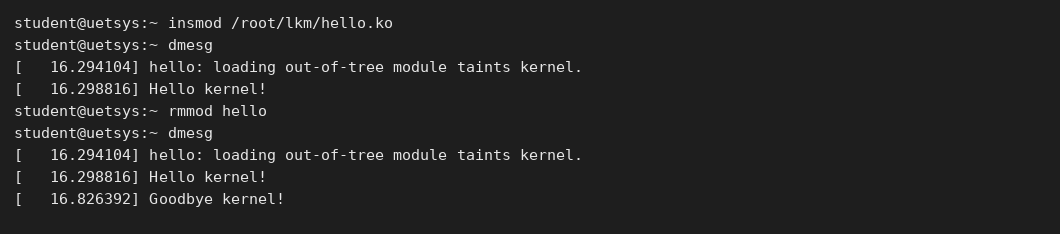
\includegraphics[width=\linewidth]{figs/b1.png}
\end{center}
\subsection{Nhận xét}
Hai macro \texttt{module\_init} và \texttt{module\_exit} đăng ký hàm khởi tạo
và hàm kết thúc của module với nhân. Hàm khởi tạo được gọi trong ngữ cảnh của
tiến trình \texttt{insmod}, trả về 0 báo nạp thành công. \texttt{printk} với mức
\texttt{KERN\_INFO} đưa thông điệp vào bộ đệm log của nhân, xem được bằng
\texttt{dmesg}. Dòng \texttt{taints kernel} là cảnh báo thông thường khi nạp
module ngoài cây nguồn chính thống, không ảnh hưởng tới chức năng.
Khai báo \texttt{MODULE\_LICENSE("GPL")} là bắt buộc để tránh nhân bị đánh dấu
\emph{tainted} do giấy phép.

% ================= BÀI 2 =================
\section{Bài 2 --- Module \texttt{hello\_param} (tham số module)}
\subsection{Mục tiêu}
Module nhận hai tham số dòng lệnh: \texttt{whom} (chuỗi ký tự, mặc định
\texttt{"world"}) và \texttt{howmany} (số nguyên, mặc định 1). Khi nạp, module
in lời chào đúng \texttt{howmany} lần; khi gỡ, in lời tạm biệt.
\subsection{Mã nguồn (\texttt{b2/hello\_param.c})}
\lstinputlisting[style=ccode]{report_code/b2/hello_param.c}
\subsection{Các bước thực hiện}
\begin{lstlisting}[style=bashcode]
sudo insmod /root/lkm/hello_param.ko whom=UET howmany=3
dmesg | tail -5
sudo rmmod hello_param
dmesg | tail -2
\end{lstlisting}
\subsection{Kết quả}
\begin{center}
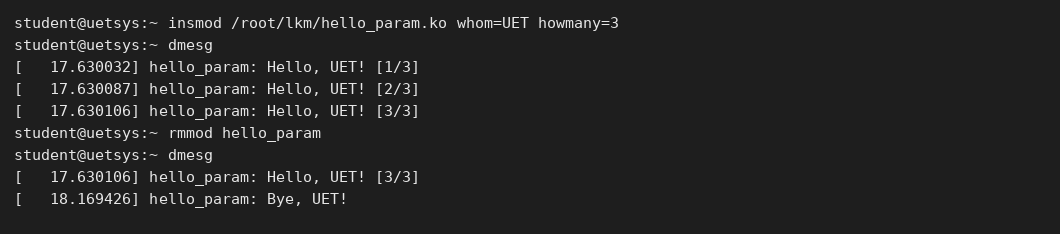
\includegraphics[width=\linewidth]{figs/b2.png}
\end{center}
\subsection{Nhận xét}
Macro \texttt{module\_param(tên, kiểu, quyền)} biến một biến toàn cục thành
tham số có thể truyền khi \texttt{insmod}. Kiểu \texttt{charp} dùng cho chuỗi,
\texttt{int} dùng cho số nguyên; quyền \texttt{0644} cho phép đọc tham số qua
sysfs. Chương trình có kiểm tra biên (\texttt{howmany < 1}) để tránh vòng lặp
rỗng hoặc hành vi không xác định khi người dùng truyền giá trị không hợp lệ.

% ================= BÀI 3 =================
\section{Bài 3 --- In dãy số và tính tổng bình phương}
\subsection{Mục tiêu}
Module nhận tham số \texttt{n} (mặc định 1). Khi nạp: in các số nguyên từ 1
đến \texttt{n} và in tổng bình phương của chúng. Khi gỡ: in thông điệp
\texttt{Done with n=\textless giá trị\textgreater}.
\subsection{Mã nguồn (\texttt{b3/b3.c})}
\lstinputlisting[style=ccode]{report_code/b3/b3.c}
\subsection{Các bước thực hiện}
\begin{lstlisting}[style=bashcode]
sudo insmod /root/lkm/b3.ko n=5
dmesg | tail -8
sudo rmmod b3
dmesg | tail -2
\end{lstlisting}
\subsection{Kết quả}
\begin{center}
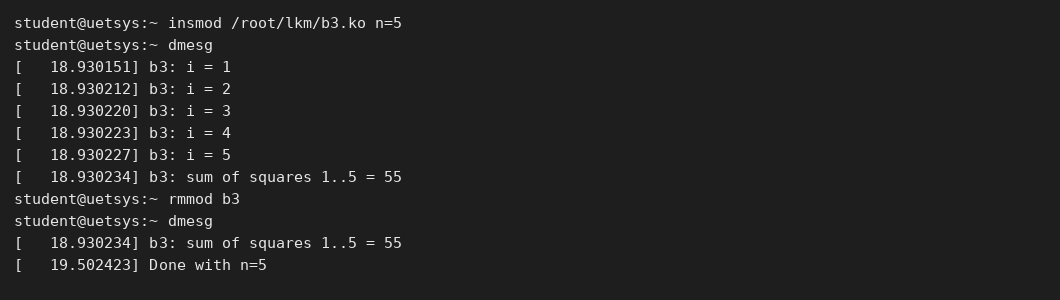
\includegraphics[width=\linewidth]{figs/b3.png}
\end{center}
\subsection{Nhận xét}
Với \texttt{n = 5}, log ghi nhận đầy đủ dãy \texttt{i = 1..5} và tổng bình
phương $1^2+2^2+3^2+4^2+5^2 = 55$, trùng với công thức
$\sum_{i=1}^{n} i^2 = n(n+1)(2n+1)/6$. Biến tích lũy dùng kiểu
\texttt{long long} (in bằng \texttt{\%lld}) để tránh tràn số khi \texttt{n}
lớn. Khi gỡ, module đọc lại giá trị hiện tại của \texttt{n} để in ra, cho thấy
tham số module tồn tại suốt vòng đời của module.

% ================= BÀI 4 =================
\section{Bài 4 --- Module \texttt{hello\_array} (tham số mảng)}
\subsection{Mục tiêu}
Module nhận tham số mảng số nguyên \texttt{nums} (tối đa 10 phần tử). Khi nạp,
in từng phần tử và tổng của mảng. Khi gỡ, in thông điệp
\texttt{hello\_array: unloaded}.
\subsection{Mã nguồn (\texttt{b4/hello\_array.c})}
\lstinputlisting[style=ccode]{report_code/b4/hello_array.c}
\subsection{Các bước thực hiện}
\begin{lstlisting}[style=bashcode]
sudo insmod /root/lkm/hello_array.ko nums=1,2,3,4,5
dmesg | tail -8
sudo rmmod hello_array
dmesg | tail -2
\end{lstlisting}
\subsection{Kết quả}
\begin{center}
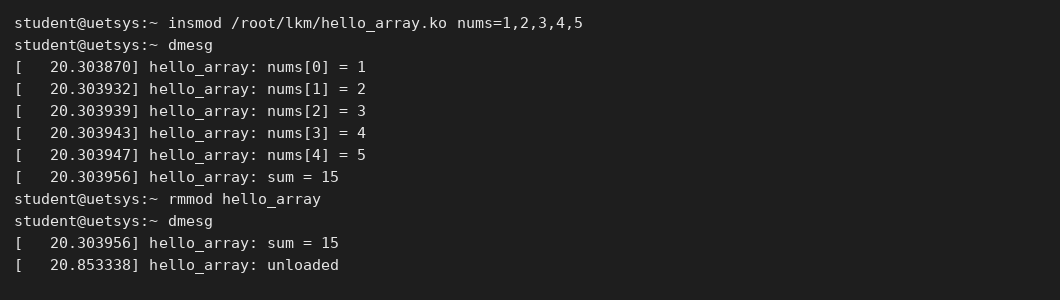
\includegraphics[width=\linewidth]{figs/b4.png}
\end{center}
\subsection{Nhận xét}
Macro \texttt{module\_param\_array} nhận danh sách giá trị cách nhau bằng dấu
phẩy trên dòng lệnh \texttt{insmod}; con trỏ \texttt{\&nums\_argc} nhận số phần
tử thực tế người dùng truyền vào. Chương trình xử lý đầy đủ ba trường hợp:
quá 10 phần tử (cắt bớt), không truyền gì (dùng mặc định \texttt{\{0\}}), và
trường hợp thông thường. Với đầu vào \texttt{1,2,3,4,5}, tổng ghi nhận là 15,
chính xác.

% ================= BÀI 5 =================
\section{Bài 5 --- Module \texttt{hello\_multi} (nhiều file nguồn)}
\subsection{Mục tiêu}
Xây dựng module gồm hai file nguồn: \texttt{main.c} chứa hàm khởi tạo/kết thúc
và gọi hàm từ file phụ; \texttt{helper.c} định nghĩa hàm
\texttt{helper\_greet()} in log. Khi nạp, module in thông điệp loaded rồi gọi
hàm phụ trợ; khi gỡ, in thông điệp unloaded.
\subsection{Mã nguồn}
\lstinputlisting[style=ccode]{report_code/b5/helper.h}
\lstinputlisting[style=ccode]{report_code/b5/helper.c}
\lstinputlisting[style=ccode]{report_code/b5/main.c}
File \texttt{Makefile} khai báo liên kết hai đối tượng thành một module:
\begin{lstlisting}[style=bashcode]
obj-m += hello_multi.o
hello_multi-objs := main.o helper.o
\end{lstlisting}
\subsection{Các bước thực hiện}
\begin{lstlisting}[style=bashcode]
sudo insmod /root/lkm/hello_multi.ko
dmesg | tail -3
sudo rmmod hello_multi
dmesg | tail -2
\end{lstlisting}
\subsection{Kết quả}
\begin{center}
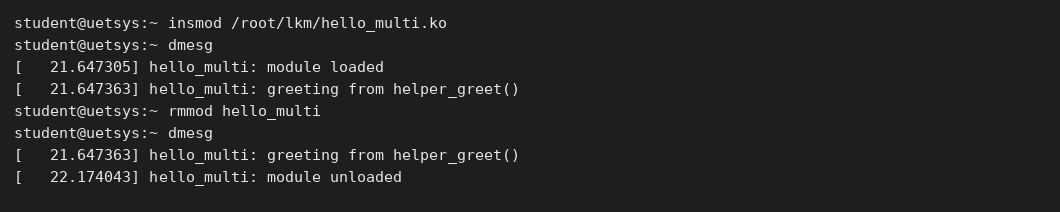
\includegraphics[width=\linewidth]{figs/b5.png}
\end{center}
\subsection{Nhận xét}
Bài này minh họa cách tổ chức module gồm nhiều file nguồn: kbuild biên dịch
riêng từng file \texttt{.c} thành \texttt{.o} rồi liên kết tĩnh thành một file
\texttt{.ko} duy nhất theo biến \texttt{<tên>-objs}. Hàm
\texttt{helper\_greet()} là liên kết tĩnh nội bộ của module (không xuất ra
ngoài), khác với cơ chế \texttt{EXPORT\_SYMBOL} dùng chung giữa các module ở
Bài 8. Log cho thấy đúng thứ tự: thông điệp loaded trước, lời chào từ hàm phụ
trợ sau.

% ================= BÀI 6 =================
\section{Bài 6 --- Module \texttt{hello\_proc} (thông tin tiến trình)}
\subsection{Mục tiêu}
Khi nạp module, in tên tiến trình gọi nạp (\texttt{current->comm}) và mã định
danh tiến trình (\texttt{current->pid}). Khi gỡ, in thông điệp unloaded.
\subsection{Mã nguồn (\texttt{b6/hello\_proc.c})}
\lstinputlisting[style=ccode]{report_code/b6/hello_proc.c}
\subsection{Các bước thực hiện}
\begin{lstlisting}[style=bashcode]
sudo insmod /root/lkm/hello_proc.ko
dmesg | tail -2
sudo rmmod hello_proc
dmesg | tail -2
\end{lstlisting}
\subsection{Kết quả}
\begin{center}
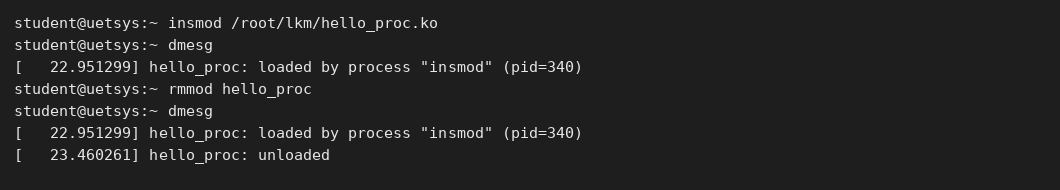
\includegraphics[width=\linewidth]{figs/b6.png}
\end{center}
\subsection{Nhận xét}
Hàm khởi tạo của module chạy trong ngữ cảnh của tiến trình người dùng gọi
\texttt{insmod}, do đó con trỏ \texttt{current} (kiểu \texttt{struct
task\_struct}, khai báo trong \texttt{linux/sched.h}) chính là tiến trình
\texttt{insmod} đó. Kết quả thực nghiệm ghi nhận đúng:
\texttt{loaded by process "insmod"}. Trường \texttt{comm} (tối đa 16 ký tự) là
tên rút gọn của tiến trình. Bài này cho thấy module nhân có thể quan sát trực
tiếp trạng thái tiến trình đang chạy.

% ================= BÀI 7 =================
\section{Bài 7 --- Module \texttt{hello\_sysfs} (tham số sysfs)}
\subsection{Mục tiêu}
Module có tham số \texttt{val} (mặc định 0) được khai báo với quyền
\texttt{0644} để cho phép đọc/ghi ngay cả khi module đang chạy, thông qua hệ
thống file sysfs.
\subsection{Mã nguồn (\texttt{b7/hello\_sysfs.c})}
\lstinputlisting[style=ccode]{report_code/b7/hello_sysfs.c}
\subsection{Các bước thực hiện}
\begin{lstlisting}[style=bashcode]
sudo insmod /root/lkm/hello_sysfs.ko val=10
dmesg | tail -2
cat /sys/module/hello_sysfs/parameters/val
echo 42 | sudo tee /sys/module/hello_sysfs/parameters/val
cat /sys/module/hello_sysfs/parameters/val
sudo rmmod hello_sysfs
dmesg | tail -2
\end{lstlisting}
\subsection{Kết quả}
\begin{center}
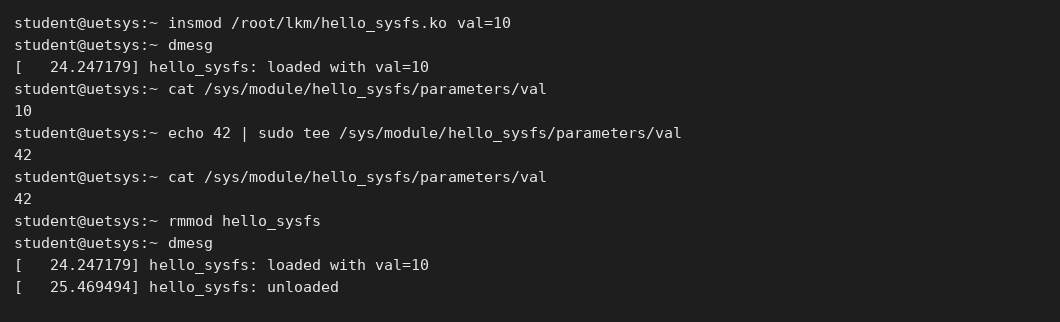
\includegraphics[width=\linewidth]{figs/b7.png}
\end{center}
\subsection{Nhận xét}
Tham số thứ ba \texttt{perm} của \texttt{module\_param} quyết định việc tạo
file sysfs tương ứng tại \texttt{/sys/module/<tên>/parameters/}: \texttt{0}
nghĩa là ẩn, \texttt{0644} nghĩa là cho phép đọc và cho phép root ghi trực
tiếp. Thực nghiệm cho thấy: sau khi nạp với \texttt{val=10}, đọc file được 10;
ghi 42 vào file rồi đọc lại được 42 mà không cần nạp lại module. Đây là cơ chế
cấu hình động module trong lúc hệ thống đang vận hành.

% ================= BÀI 8 =================
\section{Bài 8 --- Provider / Consumer (\texttt{EXPORT\_SYMBOL})}
\subsection{Mục tiêu}
Module Provider cung cấp hàm \texttt{compute\_stats} tính tổng (sum), trung
bình (avg), cực đại (max), cực tiểu (min) của một mảng số nguyên, trả kết quả
qua \texttt{struct stats\_result}, có kiểm tra tham số đầu vào. Module
Consumer dùng hàm đã xuất (export) này trên mảng mẫu
\texttt{\{10, 20, 30, 40, 50\}} và in kết quả ra log nhân.
\subsection{Mã nguồn}
\lstinputlisting[style=ccode]{report_code/b8/stats.h}
\lstinputlisting[style=ccode]{report_code/b8/provider.c}
\lstinputlisting[style=ccode]{report_code/b8/consumer.c}
\subsection{Các bước thực hiện}
\begin{lstlisting}[style=bashcode]
sudo insmod /root/lkm/provider.ko
sudo insmod /root/lkm/consumer.ko
dmesg | tail -8
sudo rmmod consumer
sudo rmmod provider
dmesg | tail -3
\end{lstlisting}
\subsection{Kết quả}
\begin{center}
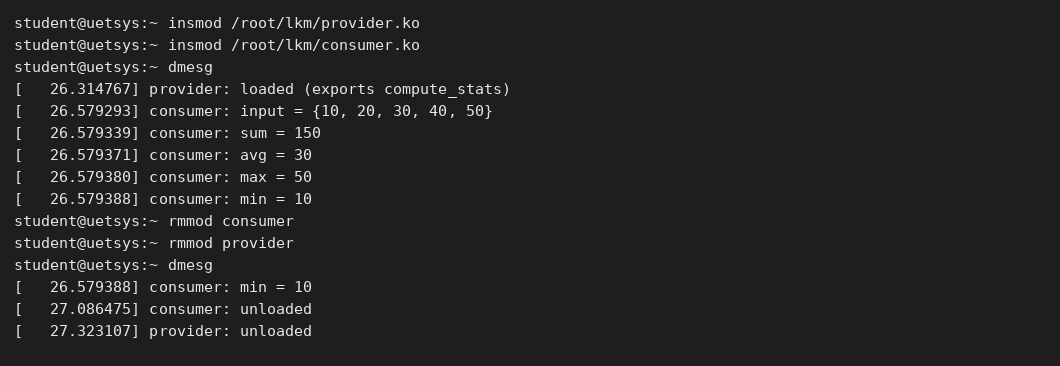
\includegraphics[width=\linewidth]{figs/b8.png}
\end{center}
\subsection{Nhận xét}
Macro \texttt{EXPORT\_SYMBOL} đưa \texttt{compute\_stats} vào bảng ký hiệu
chung của nhân, cho phép module khác liên kết động tới (thể hiện ở trường
\texttt{depends: provider} trong module Consumer). Thứ tự thao tác là bắt
buộc: phải nạp Provider trước Consumer, và gỡ Consumer trước Provider; làm
ngược lại nhân báo lỗi \texttt{Unknown symbol}. Hàm kiểm tra tính hợp lệ của
đầu vào (con trỏ \texttt{NULL}, \texttt{count <= 0}) và trả về
\texttt{-EINVAL} khi sai, tránh lỗi dereference gây oops/panic nhân. Với mảng
mẫu, kết quả thực nghiệm là \texttt{sum=150, avg=30, max=50, min=10}, hoàn toàn
chính xác.

\section{Kết luận}
Cả tám bài thực hành đều được biên dịch thành công cho nhân 5.15.163 và kiểm
chứng thực tế trên máy ảo QEMU. Nội dung đi từ cơ chế nạp/gỡ cơ bản (Bài 1),
tham số hóa module (Bài 2--4), tổ chức module nhiều file nguồn (Bài 5), truy
cập thông tin tiến trình \texttt{current} (Bài 6), cấu hình động qua sysfs
(Bài 7), đến chia sẻ hàm giữa các module bằng \texttt{EXPORT\_SYMBOL}
(Bài 8). Các kết quả trên \texttt{dmesg} đều khớp với mã nguồn và tính toán lý
thuyết, cho thấy sinh viên đã nắm vững vòng đời và cơ chế giao tiếp của
Loadable Kernel Module trong Linux.

\end{document}
